\documentclass[a4paper,11pt,twoside]{article}
%\documentclass[a4paper,11pt,twoside,se]{article}

\usepackage{UmUStudentReport}
\usepackage{verbatim}   % Multi-line comments using \begin{comment}
\usepackage{courier}    % Nicer fonts are used. (not necessary)
\usepackage{pslatex}    % Also nicer fonts. (not necessary)
\usepackage[pdftex]{graphicx}   % allows including pdf figures
\usepackage{listings}
\usepackage{pgf-umlcd}
%\usepackage{lmodern}   % Optional fonts. (not necessary)
%\usepackage{tabularx}
%\usepackage{microtype} % Provides some typographic improvements over default settings
%\usepackage{placeins}  % For aligning images with \FloatBarrier
%\usepackage{booktabs}  % For nice-looking tables
%\usepackage{titlesec}  % More granular control of sections.

% DOCUMENT INFO
% =============
\department{Department of Computing Science}
\coursename{Application Development in Java 7.5 p}
\coursecode{5DV135}
\title{RadioInfo}
\author{Lorenz Gerber ({\tt{dv15lgr@cs.umu.se}} {\tt{lozger03@student.umu.se}})}
\date{2017-01-11}
%\revisiondate{2016-01-18}
\instructor{Johan Eliasson / Jan Erik Moström / Alexander Sutherland / Filip Allberg / Adam Dahlgren Lindström}


% DOCUMENT SETTINGS
% =================
\bibliographystyle{plain}
%\bibliographystyle{ieee}
\pagestyle{fancy}
\raggedbottom
\setcounter{secnumdepth}{2}
\setcounter{tocdepth}{2}
%\graphicspath{{images/}}   %Path for images

\usepackage{float}
\floatstyle{ruled}
\newfloat{listing}{thp}{lop}
\floatname{listing}{Listing}



% DEFINES
% =======
%\newcommand{\mycommand}{<latex code>}

% DOCUMENT
% ========
\begin{document}
\lstset{language=C}
\maketitle
\thispagestyle{empty}
\newpage
\tableofcontents
\thispagestyle{empty}
\newpage

\clearpage
\pagenumbering{arabic}

\section{Introduction}
The aim of this laboration was to develop an application that uses the open web API from `Sveriges Radi' (\textit{http://sverigesradio.se/api/documentation/v2/index.html}) to present the current radio program in a graphical user interface. 

\section{Usage} 

\subsection{Compiling from command line}
The source code for the Java application `RadioInfo' was divided into the packages `model', `view', `controller' and `data\_io'. The class containing the `main' method was contained in the base directory (default package). The follwing steps were conducted to build a jar application file:

\begin{verbatim}
mkdir biuld
javac -d ./build *java model/*.java view/*.java controller/*.java ./
mode_io/*.java
cd build
jar cvfe RadioInfo.jar RadioInfoMain *.class model/ view/ controller/ ./
data_io/
\end{verbatim}

The `.jar' file is named `RadioInfo.jar' while the `main' containing class is name `RadioInfoMain'. The source code is provided in a separate tar.gz file. 



\subsection{Program Usage}
On some operating systems, double click on `RadioInfo.jar' will start the applicatoin. From the command line on OSX and -nix systems, it can be invoked by: \\
\\
\verb+java -jar RadioInfo.jar+ \\
\\
The application will start and directly show a three split window with the program table on the left, textual program description om the middle and program image on the right.
Radio programs that started before the current time are shown with white font on black blackground while programs to be broadcasted are shown with black font on white background.
To get more information about a specific program, the user can click in the table on a program. If available, the respective description and image will be shown in the middle and right side panel.
The `RadioInfo' application has a menu bar with two drop-down menus: File and Channels. In the file menu, `Reload' allows to refresh the program table by reloading it from the web, while `quit' will terminate the background update service and exit the application. In the `channels' menu, all available channels are shown and can be selected. After selection, the respective program is loaded from the net and visualized in the leftmost panel.
There is a background process running that will update the program table once every hour. 


\section{System Description}
The whole application is structured according to the \textit{Model-View-Controller} pattern. This mantra was also followed for packaging the source files. Besides the `model', `view' and `controller' package, there is also a `data\_io' package that contains the XML classes for interacting with the web API. The `RadioInfoMain' class can be found in the base directory.  


\subsection{General Structure}
In figure \ref{fig:basic}, the basic structure of the application is shown. The `main' method in \textit{RadioInfoMain Class} starts a new Swing thread, by defining an anonym \textit{runnable} method. In this method first the main data containers `channels' (\textit{ChannelListModel Class}) and `programs' (\textit{ProgramListModel Class}) are set up. Next the gui instance is started and used as method argument to the `main' (\textit{MainController}). `main' then bootstraps the whole application. 


\begin{figure}[ht!]
  \centering
  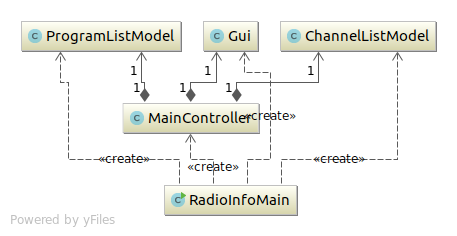
\includegraphics[width=0.8\textwidth]{basicUML.png}
  \caption{\textit{This figure shows the basic structure of the application: The main method is in the RadioInfoMain.class. It defines and starts a new thread. In this thread the two main data containers, channels (ChannelListModel class) and programs (ProgramListModel Class) are set up. Then it instantiates the gui and the MainController. The main controller takes a reference to the gui instance as construction argument. The main controller bootstraps the whole application then.}}
  \label{fig:basic}
  \end{figure}


\subsection{Data and Data Handling}

test test
\begin{figure}[p]
  \centering
  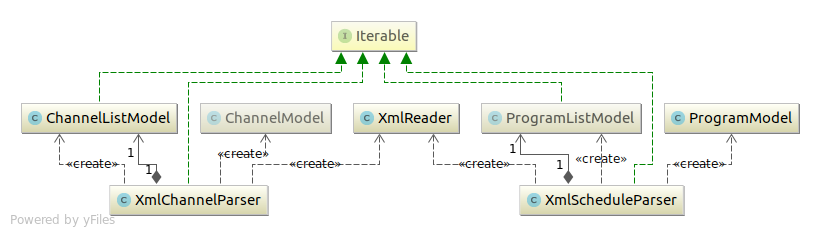
\includegraphics[width=1\textwidth]{dataModelsUML.png}
  \caption{\textit{This figure shows the data models used in RadioInfo Application}}
  \label{fig:dataModels}
\end{figure}


\subsection{The Graphical User Interface}
test testo

\begin{figure}[p]
  \centering
  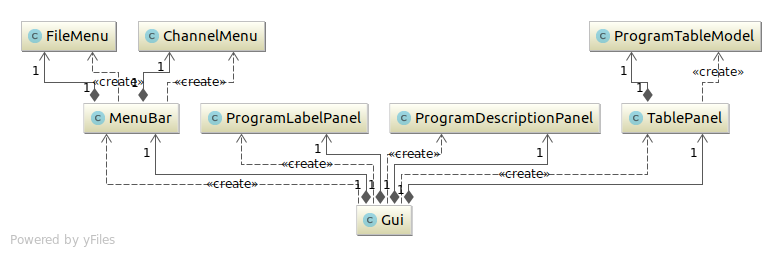
\includegraphics[width=1\textwidth]{guiUML.png}
  \caption{\textit{This figure shows the simple structure of the graphcial user interface. TablePanel, ProgramDescriptionPanel and ProgramLablePanel are all subclassed from JPanel. They are organized in a JFrame using a \textit{GridLayout} layout manager that specifies three columns and one row. The MenuBar (subclassed from JMenuBar) has two sub menus (subclassed from JMenu): FileMenu and ChannelMenu.}}
  \label{fig:gui}
\end{figure}



\subsection{Threads and Thread Safety}
The application uses separate threads for updating the data: SwingWorkers are invoked to not block the UI while pulling new data from the web API. As these operations could be potentially slow, they could be invoked again while the old one is still running. More over, user interactions such as clicking in the table potentially access the same data containers: `programs' and `channels' and `current channel'.
To make the application thread safe, synchronized methods where used. As all datacontainers get accessed through the MainController, the getters and setters in the MainController for the respective data containers were synchronized. 


\subsection{Summary of Design Patterns}
Observer-Observable
Model-View-Controller
Iterator


\section{Limitations}

\section{Testing}


\addcontentsline{toc}{section}{\refname}
\bibliography{references}

\end{document}
